
\subsection{Online shop}
\label{sec:online-shop}
As already mentioned in previous sections it is not the goal to implement a fully functional online shop as one may know it from Amazon.com or similar vendors.
Instead this one focuses on offering products, collecting feedback from the user and finally generating recommendations which will be presented to the user.

\subsubsection{General look and feel}
The key functionality of given an overview of items and recommendations is being displayed in figure~\ref{fig:onlineshop-overview}.
While random products are displayed in the left column, possible recommendations will be displayed on the right one highlighted in green.
After clicking on one of the items displayed a product view will be opened where most of the information about the selected product will be available.
The product view is responsible for receiving and interpreting the user's feedback and will be further explained in section~\ref{sec:onlineshop-feedback}.

\begin{figure}[h]
    \center
    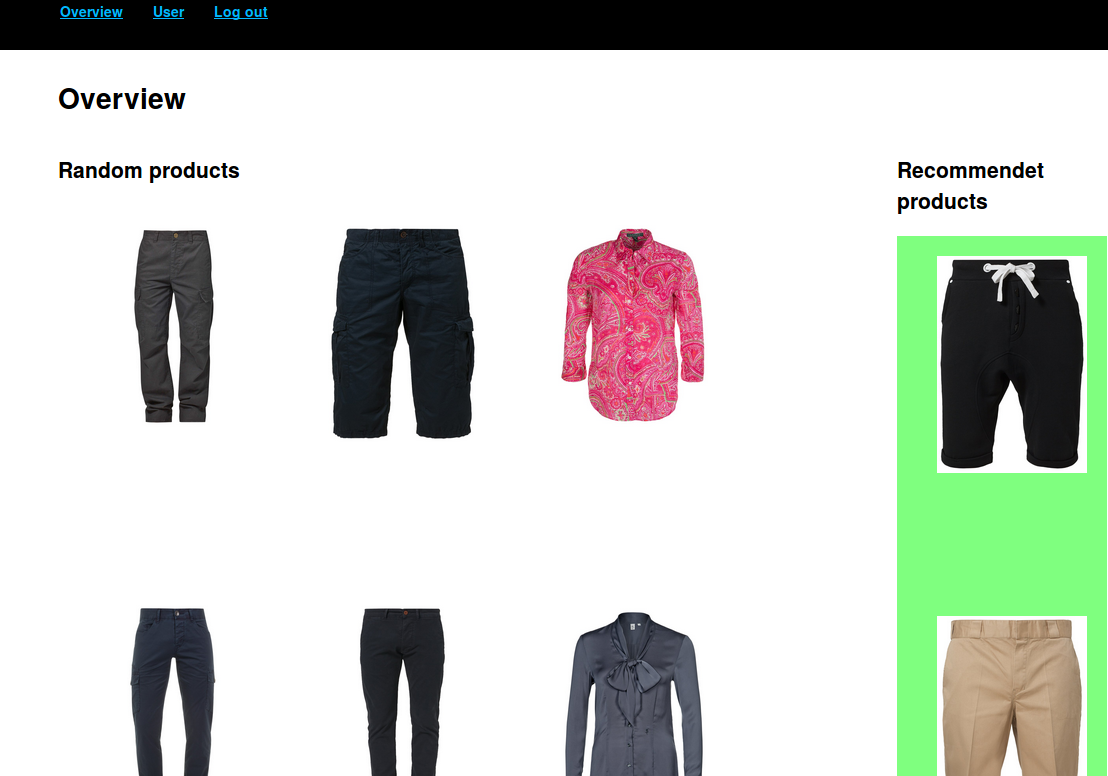
\includegraphics[scale=0.3]{inc/implementation/onlineshop/recommender_onlineshop_overview}
    \caption{Online shop overview}
    \label{fig:onlineshop-overview}
\end{figure}

\subsubsection{Feedback}
\label{sec:onlineshop-feedback}
Both implicit and explicit feedback, as introduced in section~\ref{sec:feedback}, have been implemented.
Even thought the initial task was to implement a RS which utilizes implicit feedback, explicit has been implemented as well in order to compare both methods.
There are three different ways of collecting feedback used by the online shop.
\begin{itemize}
    \item \textbf{Implicit}\hfill\\
        Whenever the user selects an item from the online-shops overview this will be interpreted as positive feedback towards the item.
    \item \textbf{Implicit timed}\hfill\\
        Instead of interpreting every item the user examines as indicator for sympathy towards the product it will be measured how long the user views the product.
        It is assumed that if the user still views the product after a pre-determined period of time he might be interested in this particular item.
    \item \textbf{Explicit binary rating}\\
        The product-view will be equipped  with a binary rating component which enables the user to explicitly like or dislike an item.
        This allows the user to remove items from the list of liked items which is not possible for the prior listed implicit methods since the user couldn't actively dislike an item.
\end{itemize}

Because implicit feedback does not require any interaction with a user there is no user interface.
For explicit feedback however the user has been given the opportunity to give a binary rating about a item whether he likes it or not.
A snippet of the user interface for explicit rating is shown in figure~\ref{fig:onlineshop-explicit-rating}.

\begin{figure}[h]
    \center
    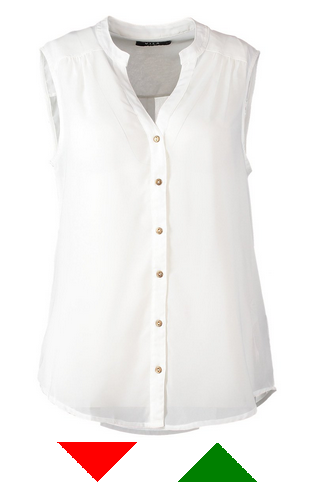
\includegraphics[scale=0.3]{inc/implementation/onlineshop/recommender-onlineshop-binary_rating}
    \caption{Binary rating of an item}
    \label{fig:onlineshop-explicit-rating}
\end{figure}

\iffalse
\subsubsection{Differences to real online-shops}
Even thought there are major differences between the implemented online shop and
\fi

%tracking through cookies
